\documentclass{beamer} %

%%%BASICS
\usepackage{fontspec}
%\usepackage[utf8]{inputenc}
\usepackage{csquotes}
\usepackage{pdfpages}

%%%START THEME SETTINGS
\usetheme{Dresden}
\usecolortheme{beaver}
\usefonttheme{professionalfonts}
\setbeamertemplate{itemize item}{\color{red}$\blacksquare$}
%%%END THEME SETTINGS

%%%START APA
%\usepackage[british]{babel}
%\usepackage[backend=biber,style=apa]{biblatex}
%\DeclareLanguageMapping{british}{british-apa}
%\addbibresource{references.bib}
%% APA citing
%% \cite{t} - Uthor und Richter, 2010
%% \textcite{t} - Uthor und Riter (2010)
%% \parencite{t} - (Uthor & Riter, 2010)
%% \parencite[Chapt.~4]{t} - (Uthor & Riter, 2010, S. 15)
%%%END APA


\title[PSY 242 Developmental Psychology]{Brain Development}
\institute[College of Staten Island]{College of Staten Island, CUNY}
\author{Xiaomeng Ma}

\date{13th September 2018}

\begin{document} 
\begin{frame}
	\titlepage
\end{frame}
%------------------------------------------------------
\begin{frame}{Introduction: Brain Basics}
\textbf{cerebral cortex, cerebellum, medulla}
\pause
    \begin{figure}
        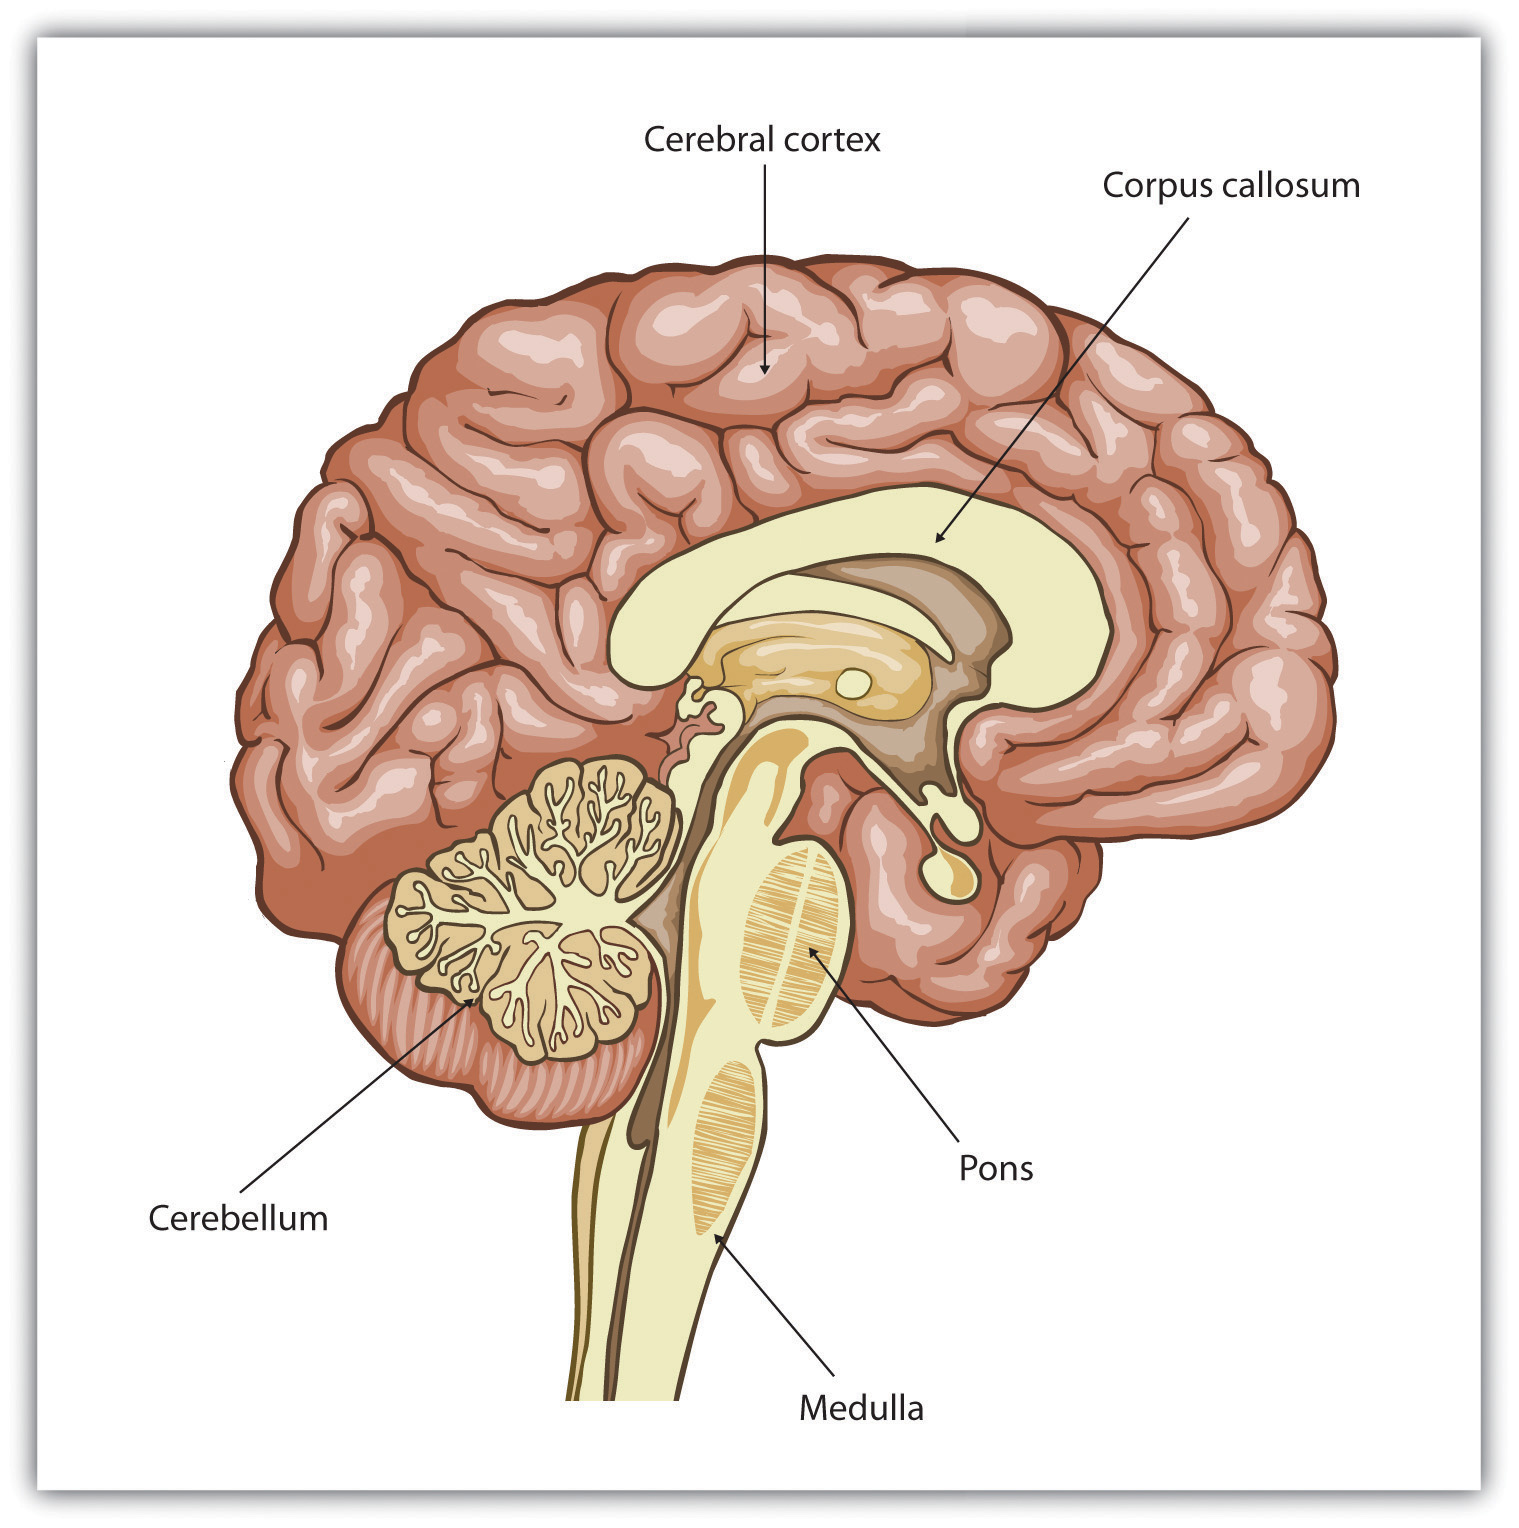
\includegraphics[height = 6cm, keepaspectratio,]{cerebro.jpg}
    \end{figure}
\end{frame}
%------------------------------------------------------
\begin{frame}{Introduction: Brain Basics}
\textbf{Neurons and Glial cells}
    \begin{figure}
        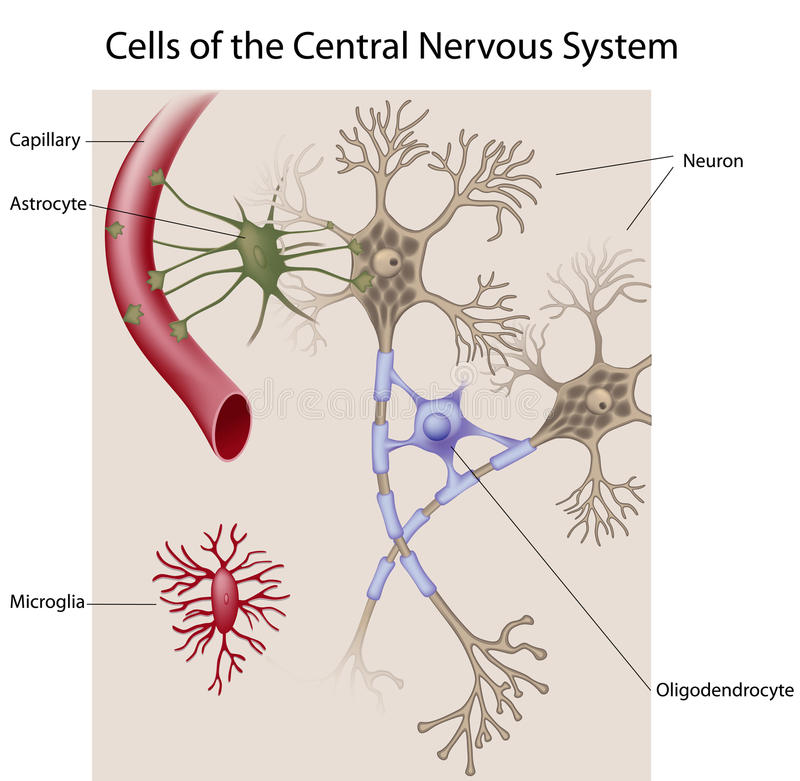
\includegraphics[height = 6cm, keepaspectratio,]{neurons-glial-cells-cns-18808418.jpg}
    \end{figure}
\end{frame}
%------------------------------------------------------
\begin{frame}{Introduction: Brain Basics}
\begin{columns}
\begin{column}{0.65\textwidth}
   \begin{figure}
       \centering
       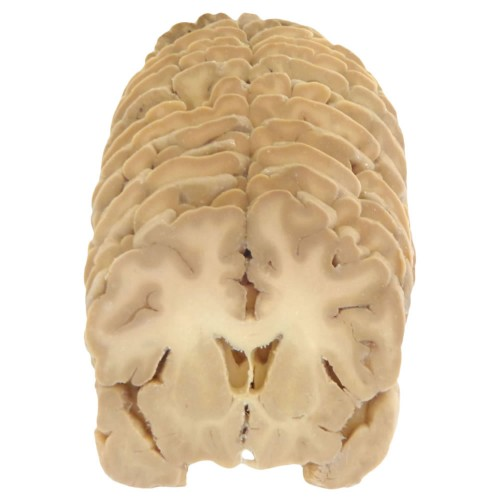
\includegraphics[height = 6cm, keepaspectration]{image_580babe38498c_nvs-042a-2-500x500.jpg}
   \end{figure}
\end{column}
\begin{column}{0.35\textwidth}  %%<--- here
    \begin{figure}
        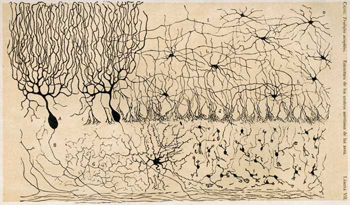
\includegraphics[width=\textwidth, height = 6cm]{CajalCerebellum.jpg}
    \end{figure}
\end{column}
\end{columns}
\end{frame}
%------------------------------------------------------
\begin{frame}{Fun Facts}
\begin{itemize}
    \item Camillo Golgi invented a silver staining technique in 1873, now known as Golgi stain
    \pause
    \item Using this technique nerve cells with their highly branched dendrites and axon could be clearly visualised against a yellow background
    \pause
    \item Ramón y Cajal started investigating nervous system in 1887 using Golgi stain and reported that nerve cells were not continuous 
    \pause
    \item Golgi and Cajal were jointly awarded the 1906 Nobel Prize for Physiology or Medicine
\end{itemize}
\end{frame}
%------------------------------------------------------
\begin{frame}{Neurons}
\begin{columns}
\begin{column}{0.5\textwidth}
\begin{itemize}
    \item Neurons: cells are specialized for sending and receiving messages between the brain and all parts of the body, as well as within the brain itself.
\end{itemize}
\end{column}
\begin{column}{0.45\textwidth}
\begin{figure}
    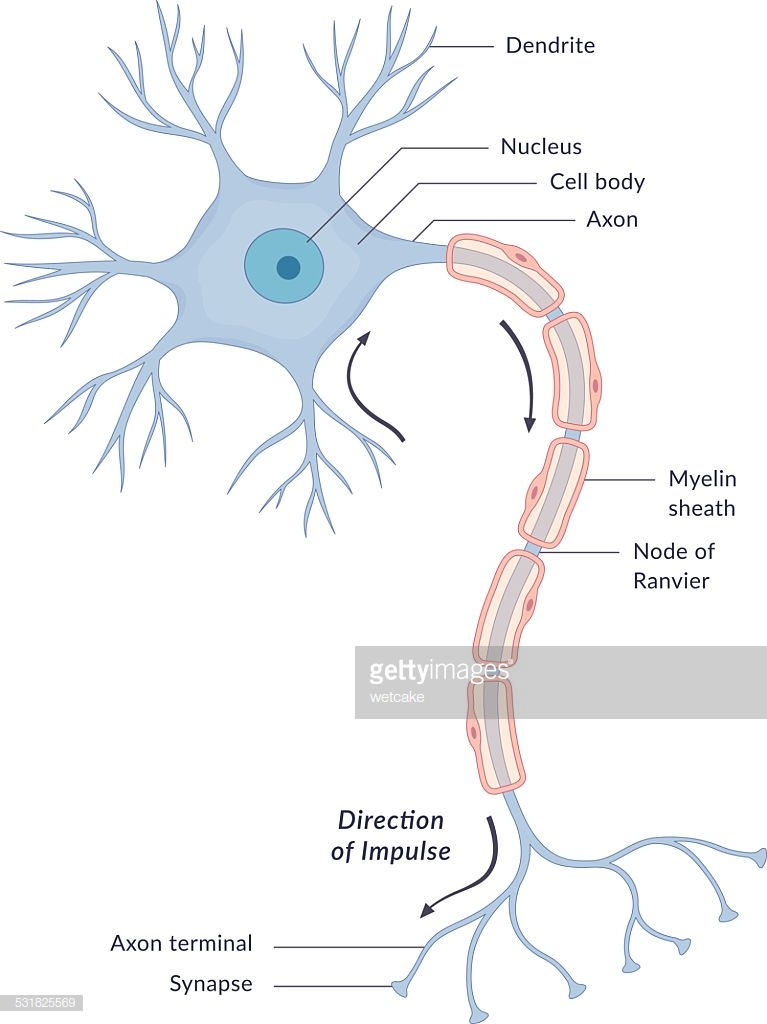
\includegraphics[width=\textwidth,height = 6cm]{531825569-1024x1024.jpg}
\end{figure}
\end{column}
\end{columns}
\end{frame}
%------------------------------------------------------
\begin{frame}{Types of Neurons}
\begin{columns}
\begin{column}{0.5\textwidth}
\begin{itemize}
    \item Sensory Neurons: transmit information from sensory receptors that detect stimuli in the external environment or within the body itself
    \item Motor Neurons: transmit information from the brain to muscles and glands
    \item Interneurons: act as intermediaries between sensory and motor neurons.
\end{itemize}
https://www.youtube.com/watch?v=uo_5l1xJnEI
\end{column}
\begin{column}{0.45\textwidth}
\begin{figure}
    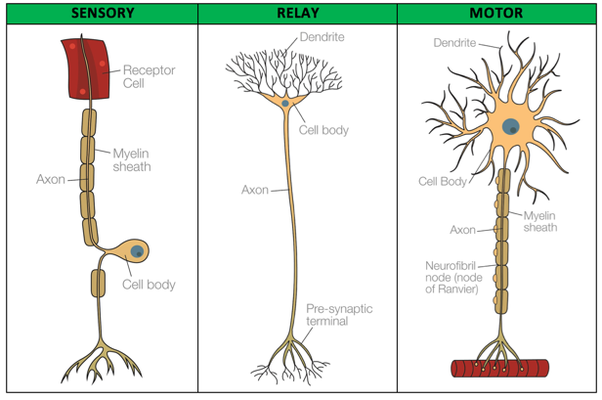
\includegraphics[width=\textwidth,height = 6cm]{main-qimg-ac1b2a998f1330d9dafc090cbb9658fd.png}
\end{figure}
\end{column}
\end{columns}
\end{frame}
%------------------------------------------------------
\begin{frame}{Components of Neurons}
\begin{columns}
\begin{column}{0.5\textwidth}
\begin{itemize}
    \item \textbf{Cell body}: which contains the basic bio- logical material that keeps the neuron functioning
    \item \textbf{Dendrites}: fibers that receive input from other cells and conduct it toward the cell body in the form of electrical impulses
    \item \textbf{Axon}: a fiber that conducts electrical signals away from the cell body to connections with other neurons.
\end{itemize}
https://www.youtube.com/watch?v=6qS83wD29PY
\end{column}
\begin{column}{0.45\textwidth}
\begin{figure}
    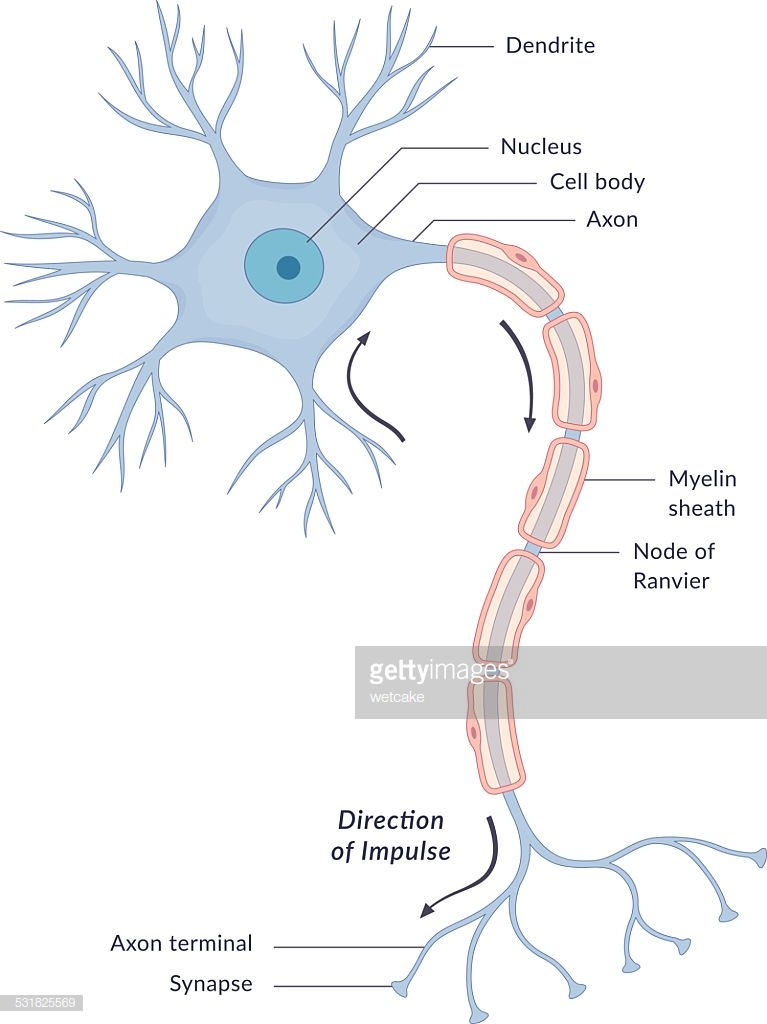
\includegraphics[width=\textwidth,height = 6cm]{531825569-1024x1024.jpg}
\end{figure}
\end{column}
\end{columns}
\end{frame}
%------------------------------------------------------
\begin{frame}{Components of Neuron}
\begin{figure}
    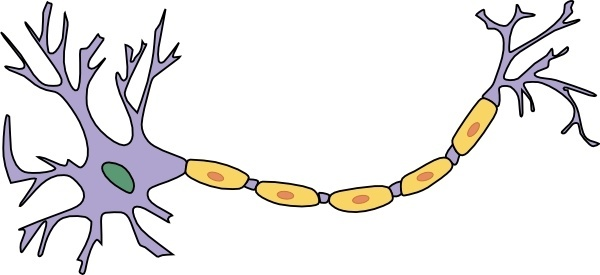
\includegraphics[width=\textwidth,height = 6cm]{neuron_with_axon_clip_art_23340.jpg}
\end{figure}
\end{frame}
%------------------------------------------------------
\begin{frame}{Components of Neuron}
\begin{figure}
    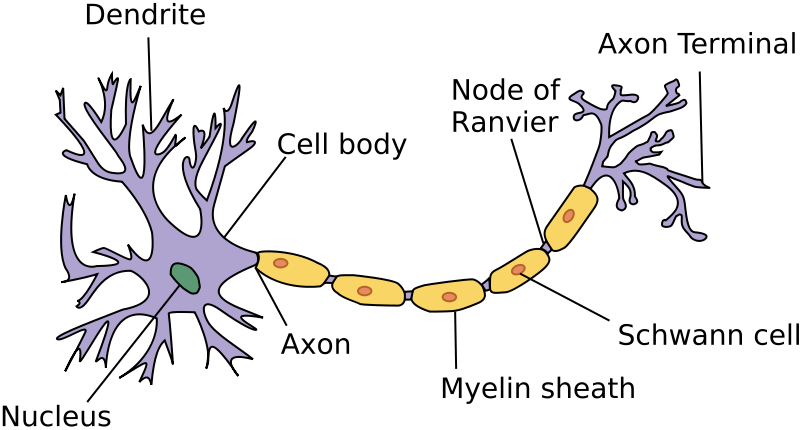
\includegraphics[width=\textwidth,height = 6cm]{800px-Neuron.svg.png}
\end{figure}
\end{frame}
%------------------------------------------------------
\begin{frame}{Glial Cells}
\begin{columns}
\begin{column}{0.5\textwidth}
\begin{itemize}
    \item \textbf{Glial Cells}:brain white matter, cells in the brain that provide a variety of critical supportive functions
    \item \textbf{Myelin Sheath}: a fatty sheath that forms around certain axons in the body and increases the speed and efficiency of information transmission
\end{itemize}
\end{column}
\begin{column}{0.45\textwidth}
\begin{figure}
    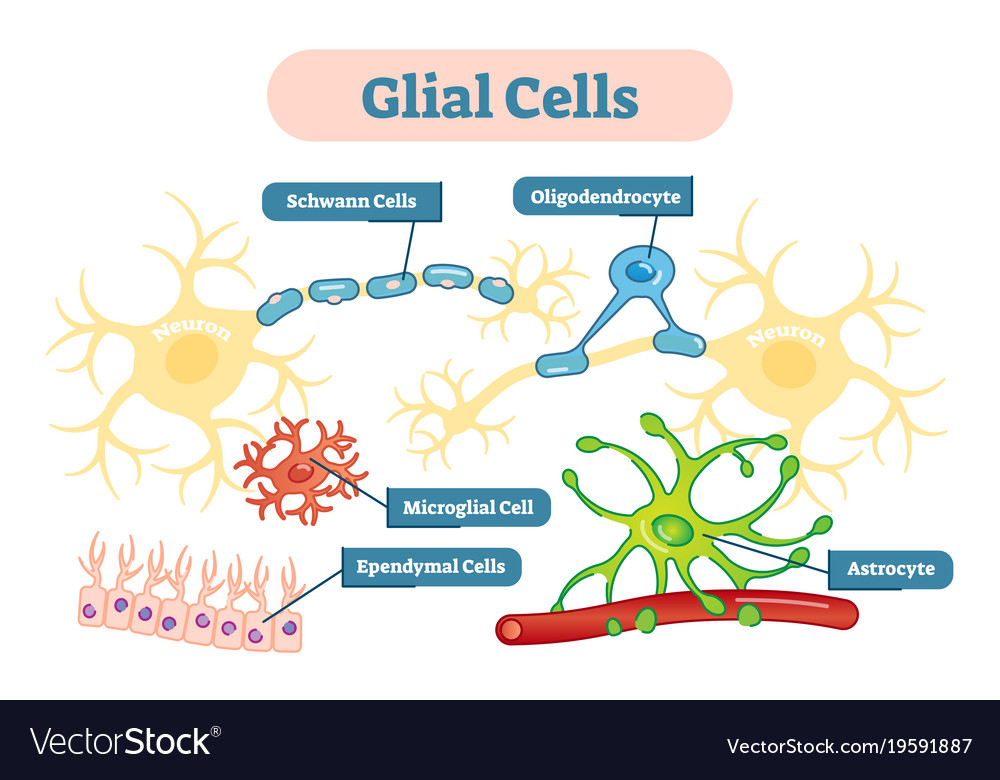
\includegraphics[width=\textwidth,height = 6cm]{nervous-system-glial-cells-schematic-diagram-vector-19591887.jpg}
\end{figure}
\end{column}
\end{columns}
\end{frame}
%------------------------------------------------------
\begin{frame}{Cortex}
\begin{columns}
\begin{column}{0.45\textwidth}
\begin{itemize}
    \item Cerebral Cortex: the “gray matter” of the brain that plays a primary role in what is thought to be particularly humanlike functioning, from seeing and hearing to writing to feeling emotion
    \item Lobes: major areas of the cortex associated with general categories of behavior
\begin{itemize}
    \item Frontal Lobe
    \item Parietal Lobe
    \item Temporal Lobe
    \item Occipital Lobe
\end{itemize}
\end{itemize}
\end{column}
\begin{column}{0.65\textwidth}
\begin{figure}
    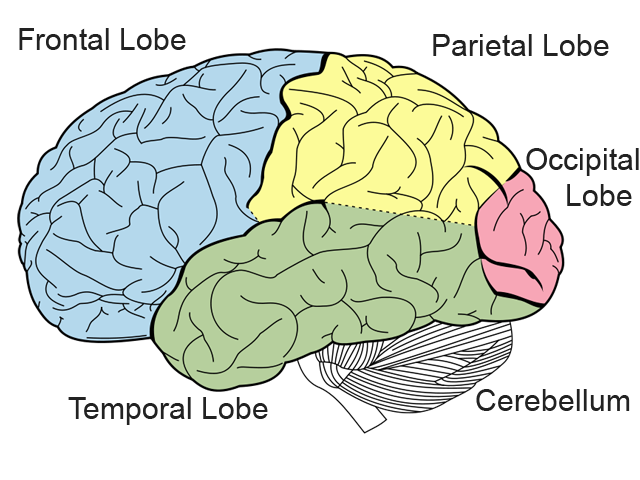
\includegraphics[width=\textwidth,height = 6cm]{6645d46c_151a22e0018__8000_00008559.png}
\end{figure}
\end{column}
\end{columns}
\end{frame}
%------------------------------------------------------
\begin{frame}{Cortex}
\begin{figure}
    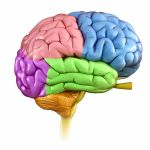
\includegraphics[width=\textwidth,height = 8cm]{brain-lobe-function-diagram-unique-brain-anatomy-the-4-lobes-structures-and-functions-150x150.jpg}
\end{figure}
\end{frame}
%------------------------------------------------------
\begin{frame}{Cortex}
\begin{itemize}
    \item Frontal Lobe: associated with organizing behavior; the one that is thought responsible for the human ability to plan ahead
    \item Parietal Lobe: Spatial Information processing and integration of different sensory modalities
    \item Temporal Lobe: Memory, visual recognition, speech and language, and the processing of emotion and auditory information. 
    \item Occipital Lobe: Visual information
\end{itemize}
\end{frame}
%------------------------------------------------------
\begin{frame}{Cortex}
\begin{figure}
    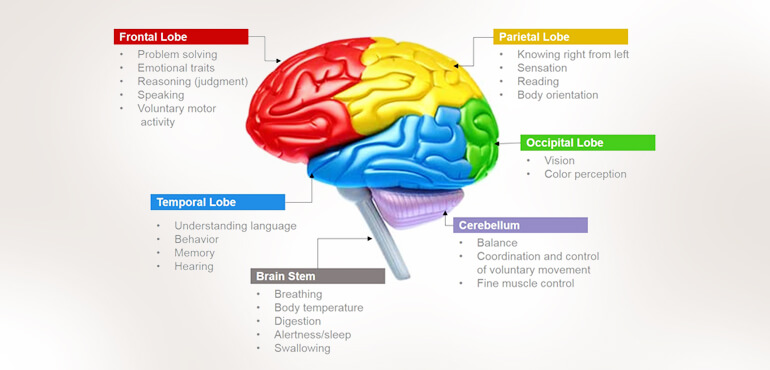
\includegraphics[height = 8cm, keepaspectration]{human-brain-functions.jpg}
\end{figure}
\end{frame}
%------------------------------------------------------
\begin{frame}{Cerebral lateralization}
\begin{columns}
\begin{column}{0.4\textwidth}
\begin{itemize}
    \item Cerebral lateralization: the specialization of the hemispheres of the brain for different modes of processing
    \item Corpus callosum: a dense tract of nerve fibers that enable the two hemispheres of the brain to communicate
\end{itemize}
\end{column}
\begin{column}{0.55\textwidth}
\begin{figure}
    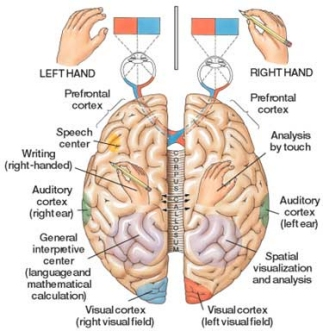
\includegraphics[height = 6cm, keepaspectration]{brain.jpg}
\end{figure}
\end{column}
\end{columns}
\end{frame}
%------------------------------------------------------
\begin{frame}{Neuron Development}
\begin{itemize}
    \item Neurogenesis: the proliferation of neurons through cell division
    \\ https://www.youtube.com/watch?v=XdN9iZWGho
    \item Neurogenesis also occurs in adult life, e.g learning
    \\ https://www.youtube.com/watch?v=ewNvcFJEHbA
    \\ https://www.youtube.com/watch?v=EP4yeyD8ktY
    \item ++ length of axons, density of dendrites
    \pause
    \item Myelination: the formation of myelin (a fatty sheath) around the axons of neurons that speeds and increases information-processing abilities
   \\  https://www.youtube.com/watch?v=zLan1UrSCxk
\end{itemize}
\end{frame}
%------------------------------------------------------
\begin{frame}{Neuron Development}
\begin{figure}
    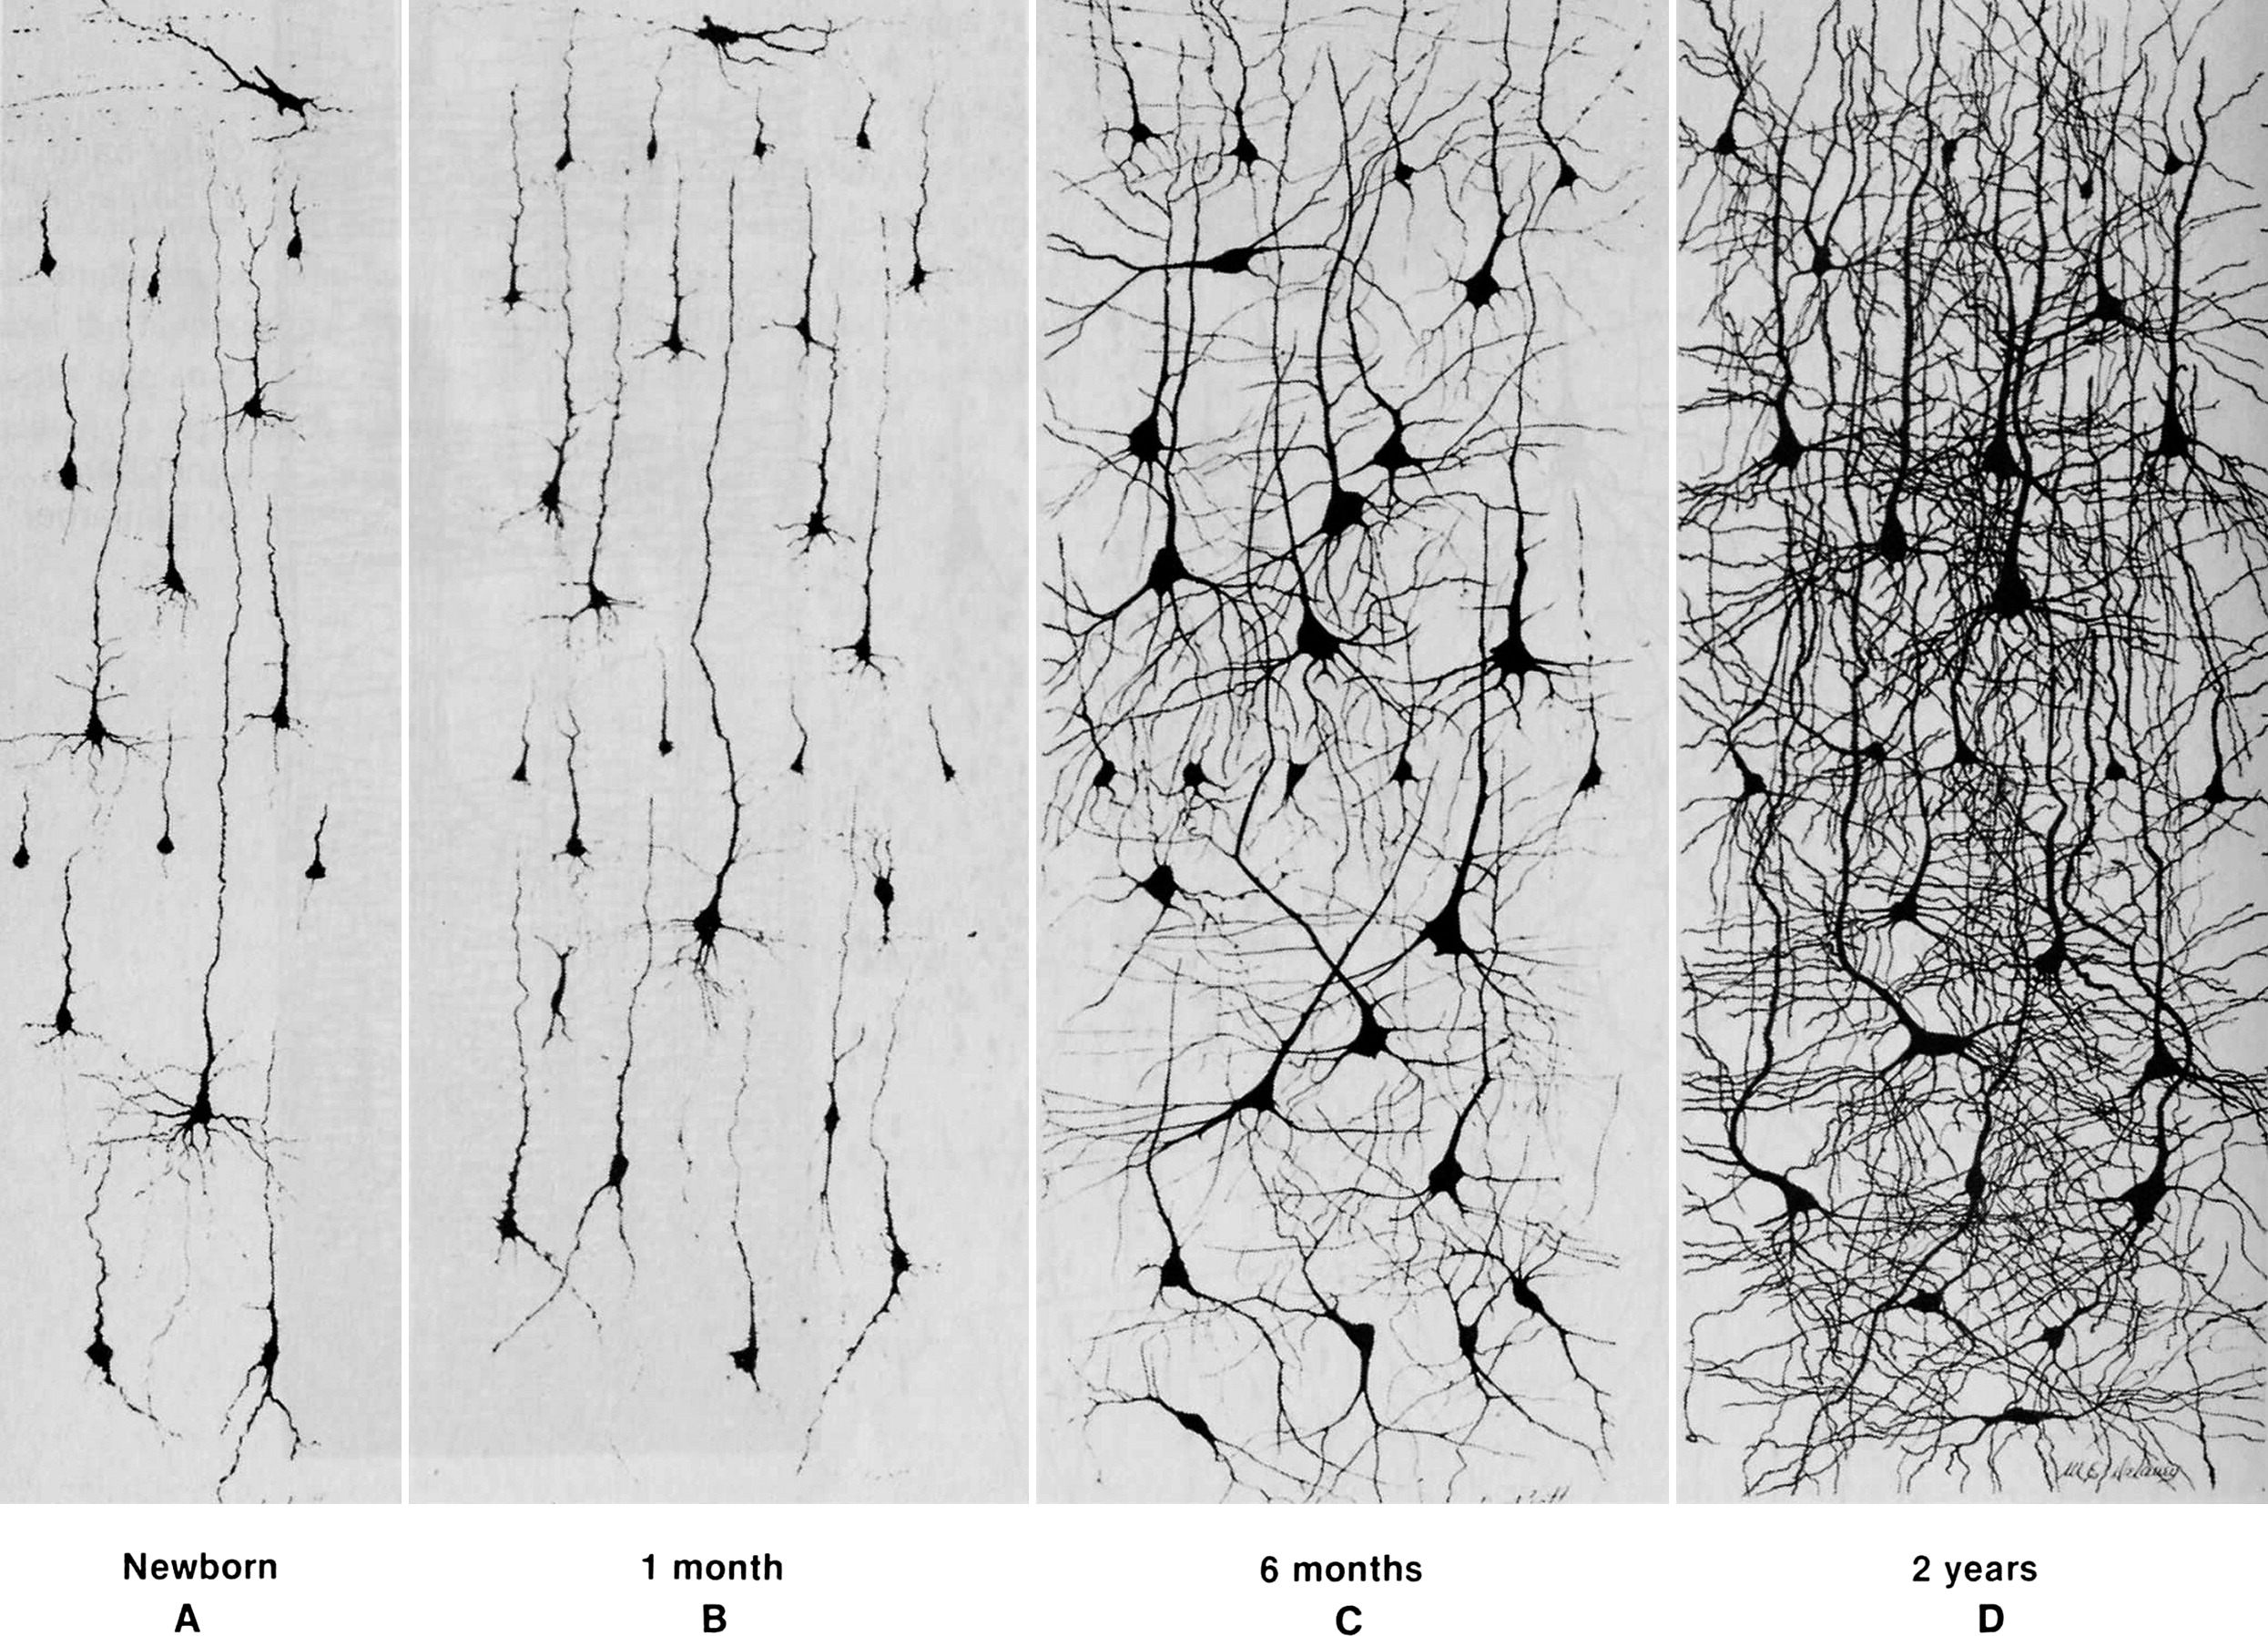
\includegraphics[height=6cm, keepaspectration]{dendrites-02.jpg}
\end{figure}
\end{frame}
%------------------------------------------------------
\begin{frame}{Neuron Development}
\begin{itemize}
    \item Synaptogenesis: the process by which neurons form synapses with other neurons, resulting in trillions of connections
    \item Synaptic pruning: the normal developmental process through which synapses that are rarely activated are eliminated
    \begin{figure}
        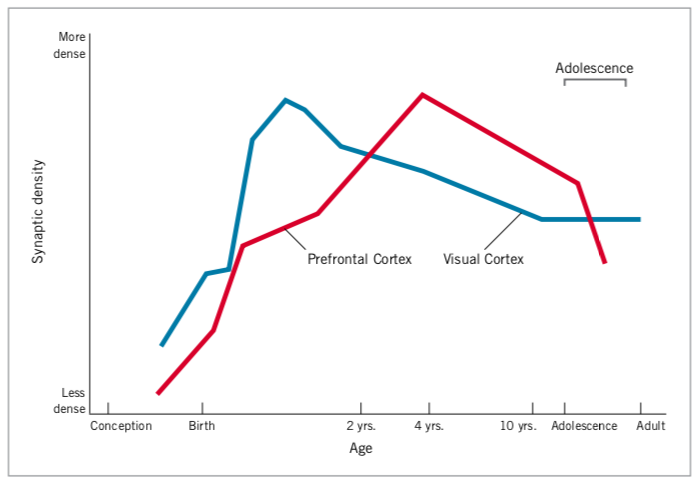
\includegraphics[height=4cm, keepaspectration]{sss.png}
    \end{figure}
\end{itemize}
\end{frame}
%------------------------------------------------------
\begin{frame}{Neuron Development}
https://bit.ly/2QsRNE6
\begin{figure}
    \centering
    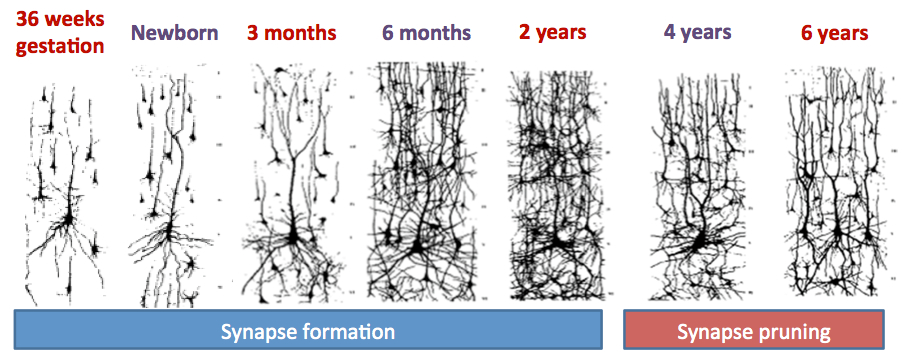
\includegraphics[width=\linewidth, keepaspectration]{brainscience.png}
\end{figure}
What if there is no prunning?
\\ https://www.youtube.com/watch?v=DrIZJnVxCbY
\end{frame}
%------------------------------------------------------
\begin{frame}{Plasticity}
\begin{itemize}
    \item Plasticiy: the capacity of the brain to be affected by experience
    \\ https://www.youtube.com/watch?v=dmEOJyWVQj4
    \item Experience-Expectant Plasticity: the process through which the normal wiring of the brain occurs in part as a result of experiences that every human who inhabits any reasonably normal environment will have
    \\ Example: https://www.youtube.com/watch?v=ySIDMU2cy0Y
    \item Sensitive Period (Critical Period): There are a few sensitive periods when the human brain is especially sensitive to particular kinds of external stimuli. (e.g Language)
    \item Brain Damage: Examples from Traumatic Brain Injury (TBI) https://www.youtube.com/watch?v=OiLBPsTRLnQ
\end{itemize}
\end{frame}
%------------------------------------------------------
\end{document}
